\documentclass[30pt, a0paper, portrait, margin=0mm, innermargin=15mm,
               blockverticalspace=15mm, colspace=15mm, subcolspace=8mm]{tikzposter} 

% Change font     
\renewcommand{\familydefault}{\sfdefault}

\definecolor{mycol}{HTML}{326E77}
\definecolorstyle{myColorStyle}{
  \colorlet{colorOne}{darkgray}
  \colorlet{colorTwo}{gray}
  \colorlet{colorThree}{gray}
}{
  % Background Colors
  \colorlet{backgroundcolor}{colorTwo!50}
  \colorlet{framecolor}{black}
  % Title Colors
  \colorlet{titlefgcolor}{black}
  \colorlet{titlebgcolor}{colorOne}
  % Block Colors
  \colorlet{blocktitlebgcolor}{mycol}
  \colorlet{blocktitlefgcolor}{white}
  \colorlet{blockbodybgcolor}{white}
  \colorlet{blockbodyfgcolor}{black}
  % Innerblock Colors
  \colorlet{innerblocktitlebgcolor}{white}
  \colorlet{innerblocktitlefgcolor}{black}
  \colorlet{innerblockbodybgcolor}{white}
  \colorlet{innerblockbodyfgcolor}{black}
  % Note colors
  \colorlet{notefgcolor}{black}
  \colorlet{notebgcolor}{white}
  \colorlet{notefrcolor}{white}
}

% LATEX PACKAGES
% --------------
  
\usepackage{graphicx}  % package for inserting images, including .pdf
\usepackage{adjustbox} % package for cropping images
\usepackage[colorlinks=true, urlcolor=red]{hyperref} % package for url and hyperlinks
\usepackage{wrapfig}
\usepackage{lmodern} %mix italic and bold
\usepackage{hyperref}% for url
\usepackage{authblk}
\usepackage{graphicx} 
\usepackage{caption}
\usepackage{mwe}
\usepackage[absolute]{textpos}

\usepackage{graphicx}

% TITLE, AUTHORS, INSTITUTE
% -------------------------
% Left logo

\title{\parbox{\linewidth}{\centering \textbf{Parasites and the eukaryotic biome - \\diversity is associated  with social rank in spotted hyena}}}

\author[1,2,*]{Emanuel~Heitlinger} \author[3]{Susana~C~Ferreira}
\author[3]{Dagmar~Thierer} \author[3]{Heribert~Hofer}
\author[3]{Marion~L~East}

\affil[1]{\Large Research Group Ecology and Evolution of molecular Parasite-Host
  Interactions, Leibniz Institute for Zoo and Wildlife
  Research (IZW), Berlin} 
\affil[2]{\Large Department of Molecular Parasitology, Humboldt
  University (HU), Berlin}
\affil[3]{\Large Department Evolutionary Ecology, Leibniz Institute for Zoo and Wildlife
  Research (IZW), Berlin}
  \affil[*]{\textbf{Correspondence:}
  \textcolor{blue} {emanuel.heitlinger@hu-berlin.de, Heitlinger@izw-berlin.de}, \textbf{Twitter: }\textcolor{blue}{@EHeitlinger} \vspace{-6ex}}


\makeatletter
\def\maketitle{\AB@maketitle}
\makeatother

% THEME SETTING
% -------------
\usetheme{Default}
\usecolorstyle{myColorStyle}
\useblockstyle{Basic}
\usebackgroundstyle{Empty}
\usetitlestyle{Empty}


% HEAD
% ----

\begin{document}

\maketitle

\begin{columns}

% ------------------------
% COLUMN 1 ---------------
  
\column{0.5}

% Context
% ----

\block{Context, Predictions and Aims}
{
  In the spotted hyena (\textit{Crocuta crocuta}), a highly
  social, female-dominated carnivore social status
  determines access to resources.\\
  \\
  \noindent
  \hspace{1cm}
  \begin{minipage}{0.5\linewidth}                  
   \begin{left}
     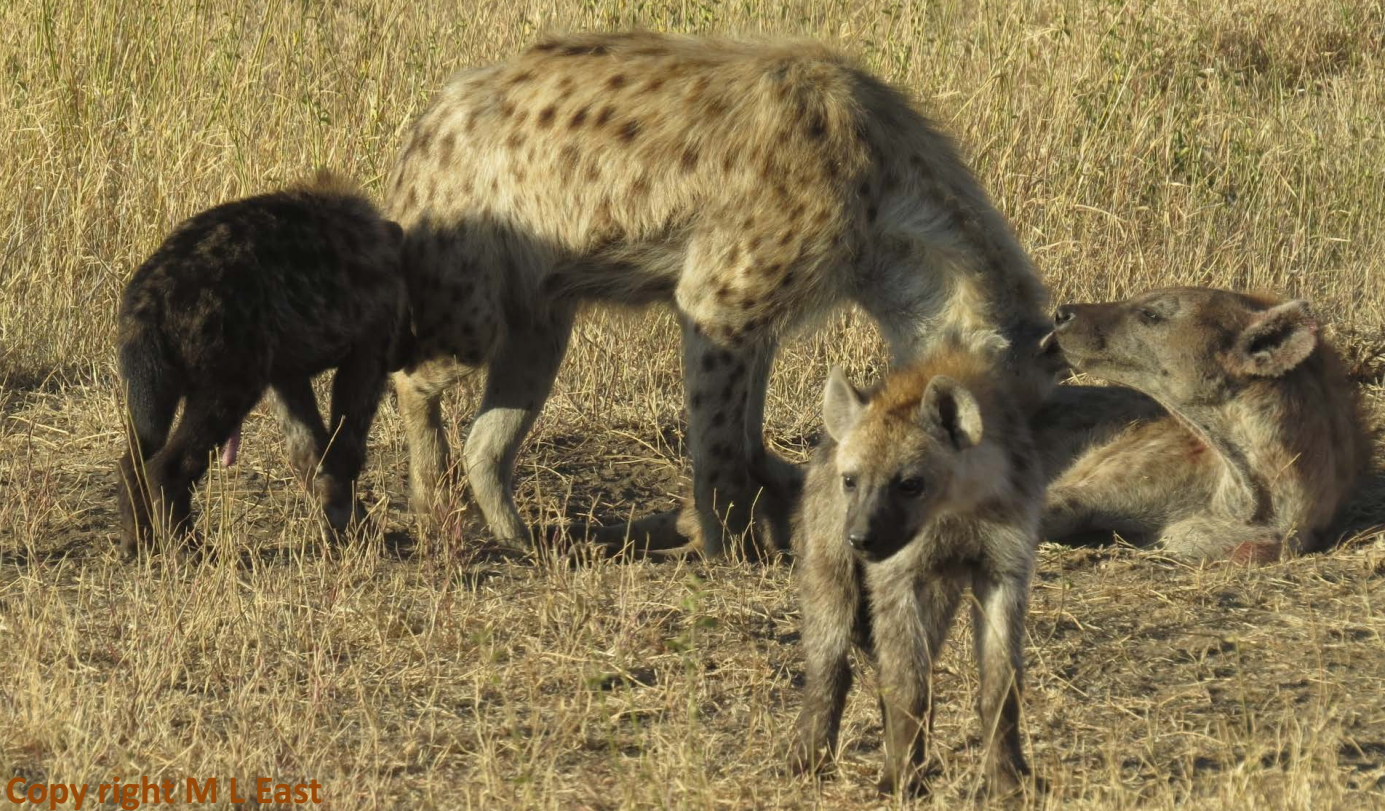
\includegraphics[width=1\linewidth]{Hyena.png}
   \end{left}
   \\\textbf{Fig 1:} Hyenas interacting at a den.
\end{minipage}
\hfill
\begin{minipage}{0.5\linewidth}
\\Predictions:
  \begin{itemize}
 \item{High species diversity is an index of ecosystem health, the
   intestinal biome of healthier, socially dominant animals should be
   more diverse than those of subordinates.}\\
 \item{Gradual colonization of the juvenile intestine after birth
   predicts lower intestinal biome diversity in juveniles than
   adults.}
 \end{itemize}
\end{minipage} 
\hfill
}      
      
\block{Results: Validation}
      {
        \begin{minipage}{0.7\linewidth}                  
          \begin{left}
            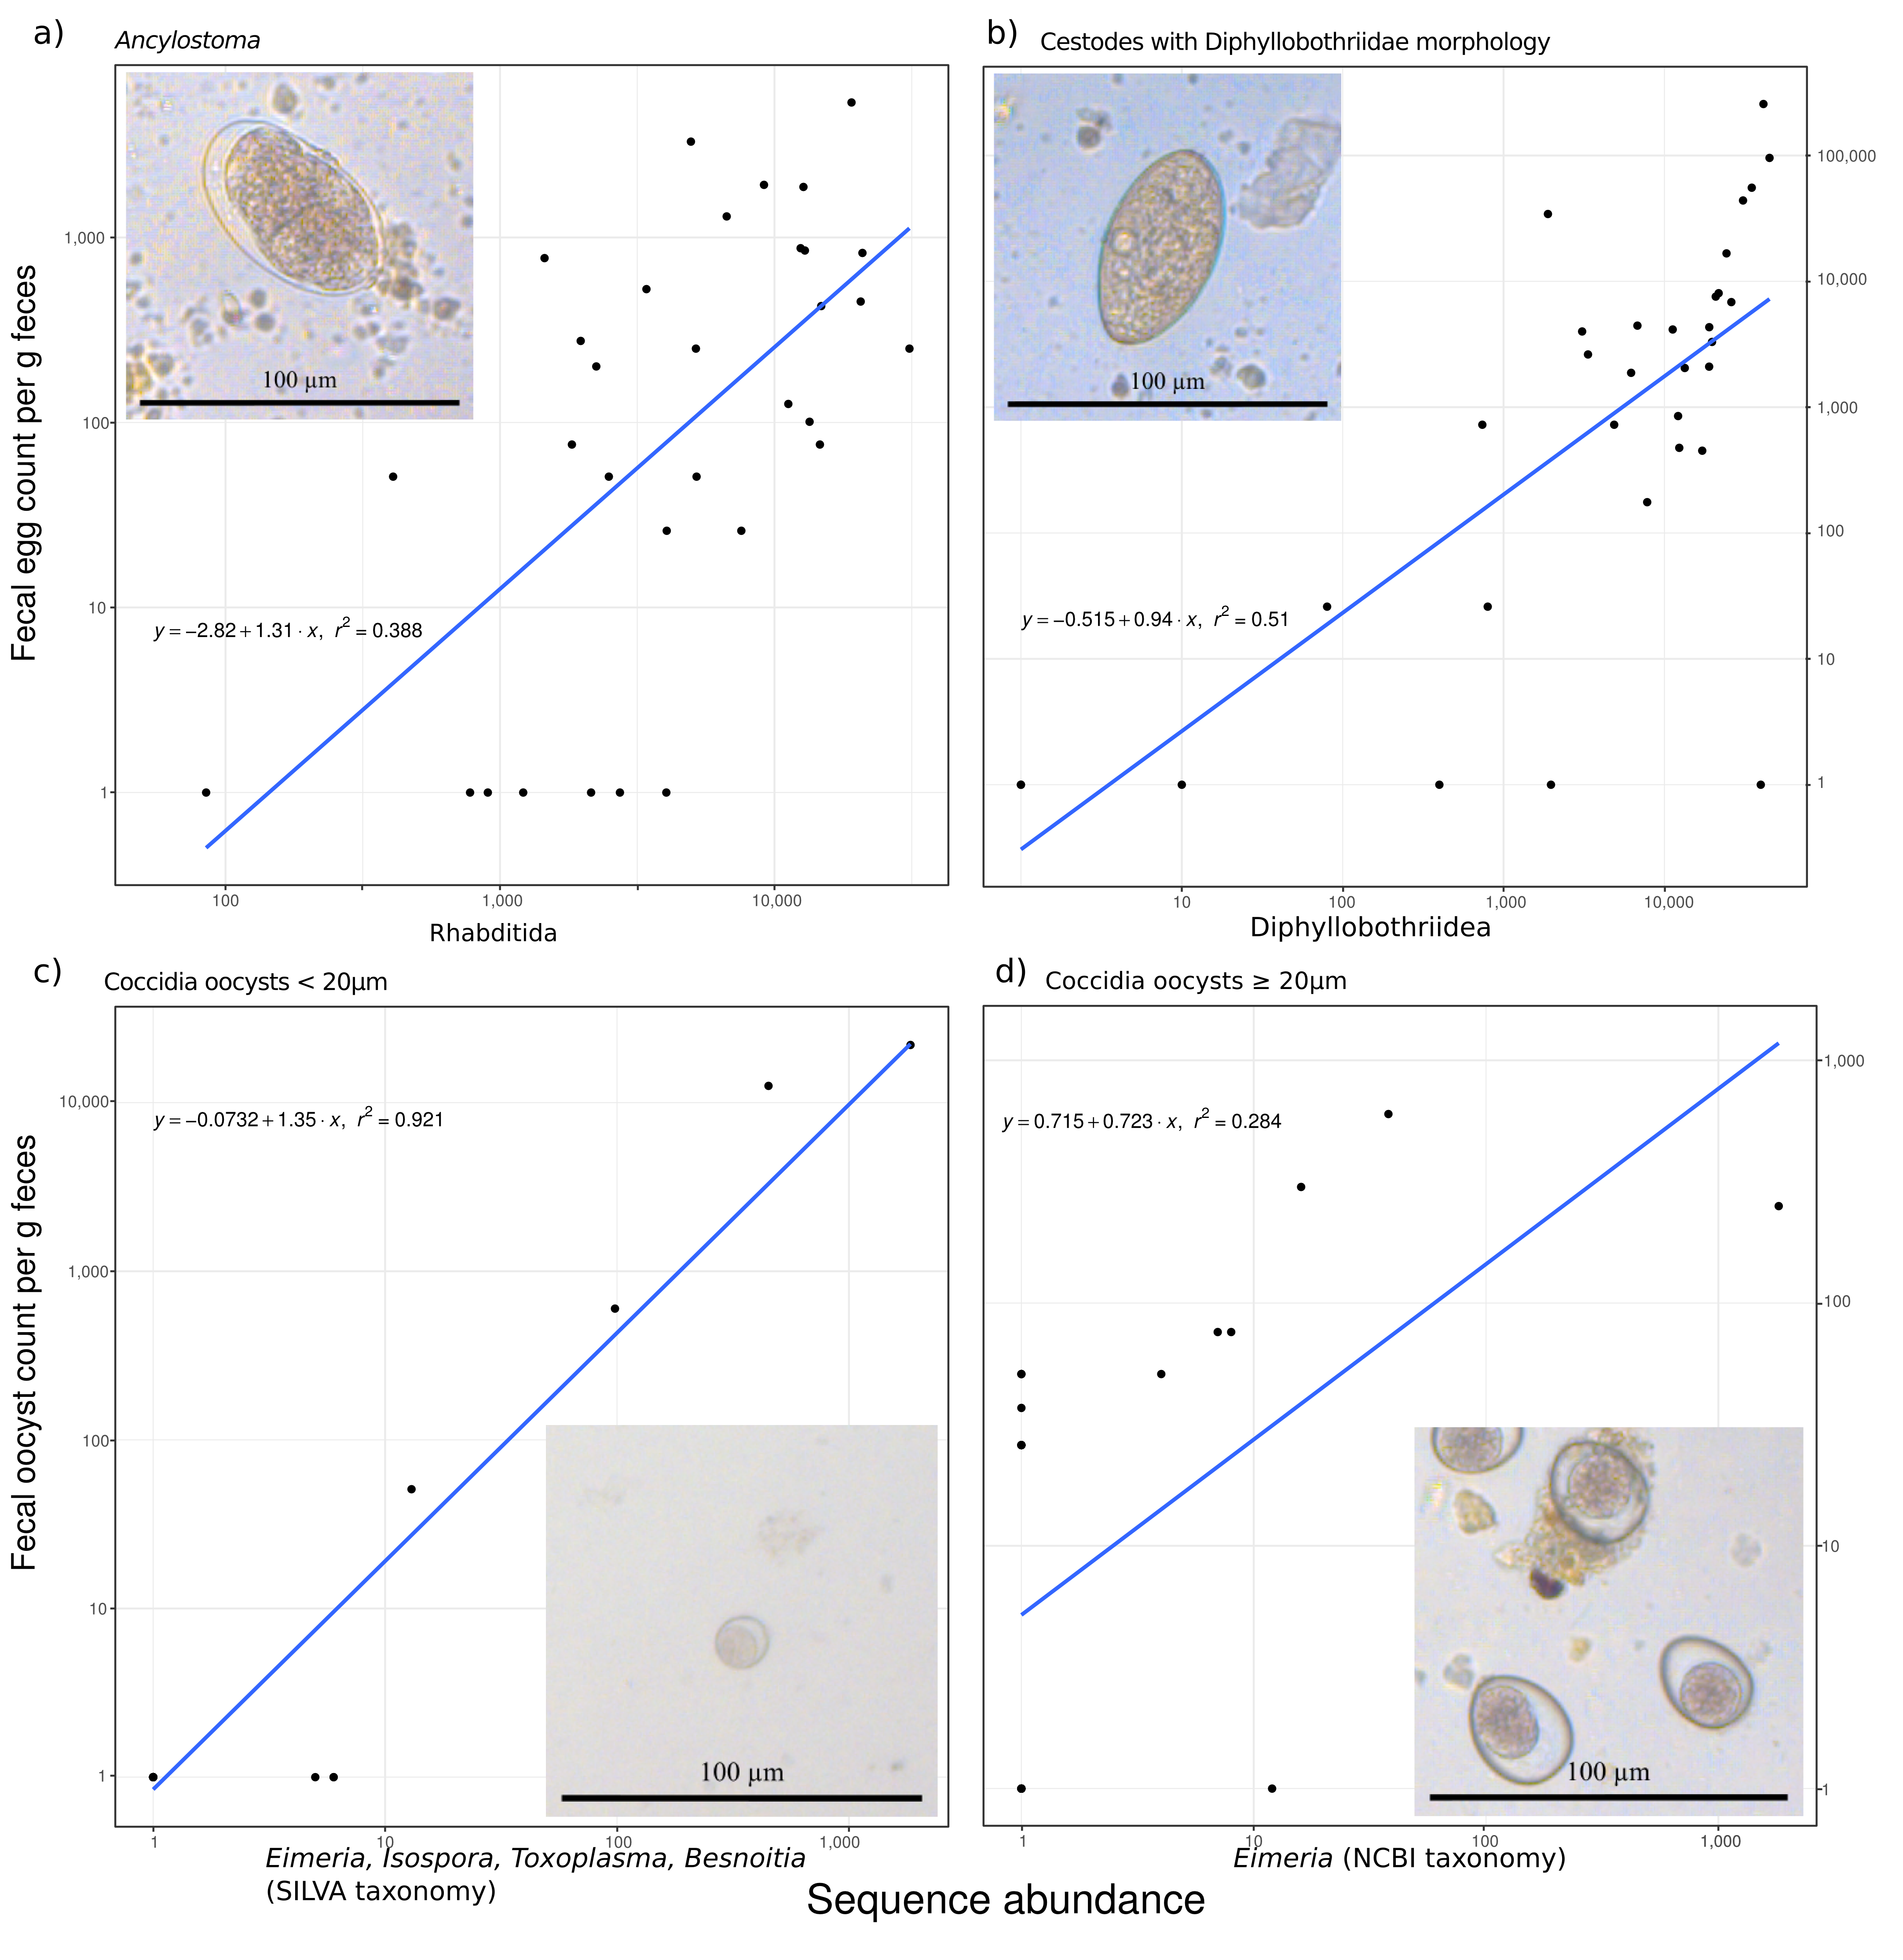
\includegraphics[scale=0.7]{Figure2_man.png}
          \end{left}
        \end{minipage}
        \hfill
        \begin{minipage}{0.3\linewidth}
          \textbf{Fig 2:} Ribosomal sequence fragments (RSVs) predict
          fecal egg or oocyst counts for (a) Ancylostoma (Rhabditida),
          (b) Diphyllobothriidae and (c and d) small and a large size
          classes of Coccidia (\textit{Eimeria}, \textit{Isospora},
          \textit{Besnoitia}, and \textit{Toxoplasma}).
          \\ \\ $\Rightarrow$
          \textbf{Quantitative assessment of eukaryotes with high
            sensitivity.}
        \end{minipage}
      }

 \block{Methods}
      {
        Study animals:
        \begin{itemize}
        \item 35 individually known adult females and 7 juveniles ($<$
          24 months) for three clans of the Serengeti ecosystem
        \item Social status categorized as above/below the median rank
        \item Parasite eggs or oocysts counted for 32 individuals
        \end{itemize}
        Amplicon sequencing:
        \begin{itemize}
        \item{48 different amplicons (4 for bacterial 16S, 44 for
          eukaryote 18S) in a multi-amplicon sequencing approach.}
        \item{Processed on a microfluidics PCR system (Fluidigm Access
          Array\textsuperscript{\textregistered})}
        \item{Data processing pipeline using RSVs [1] is available as
          an R package [2].}
        \end{itemize}
        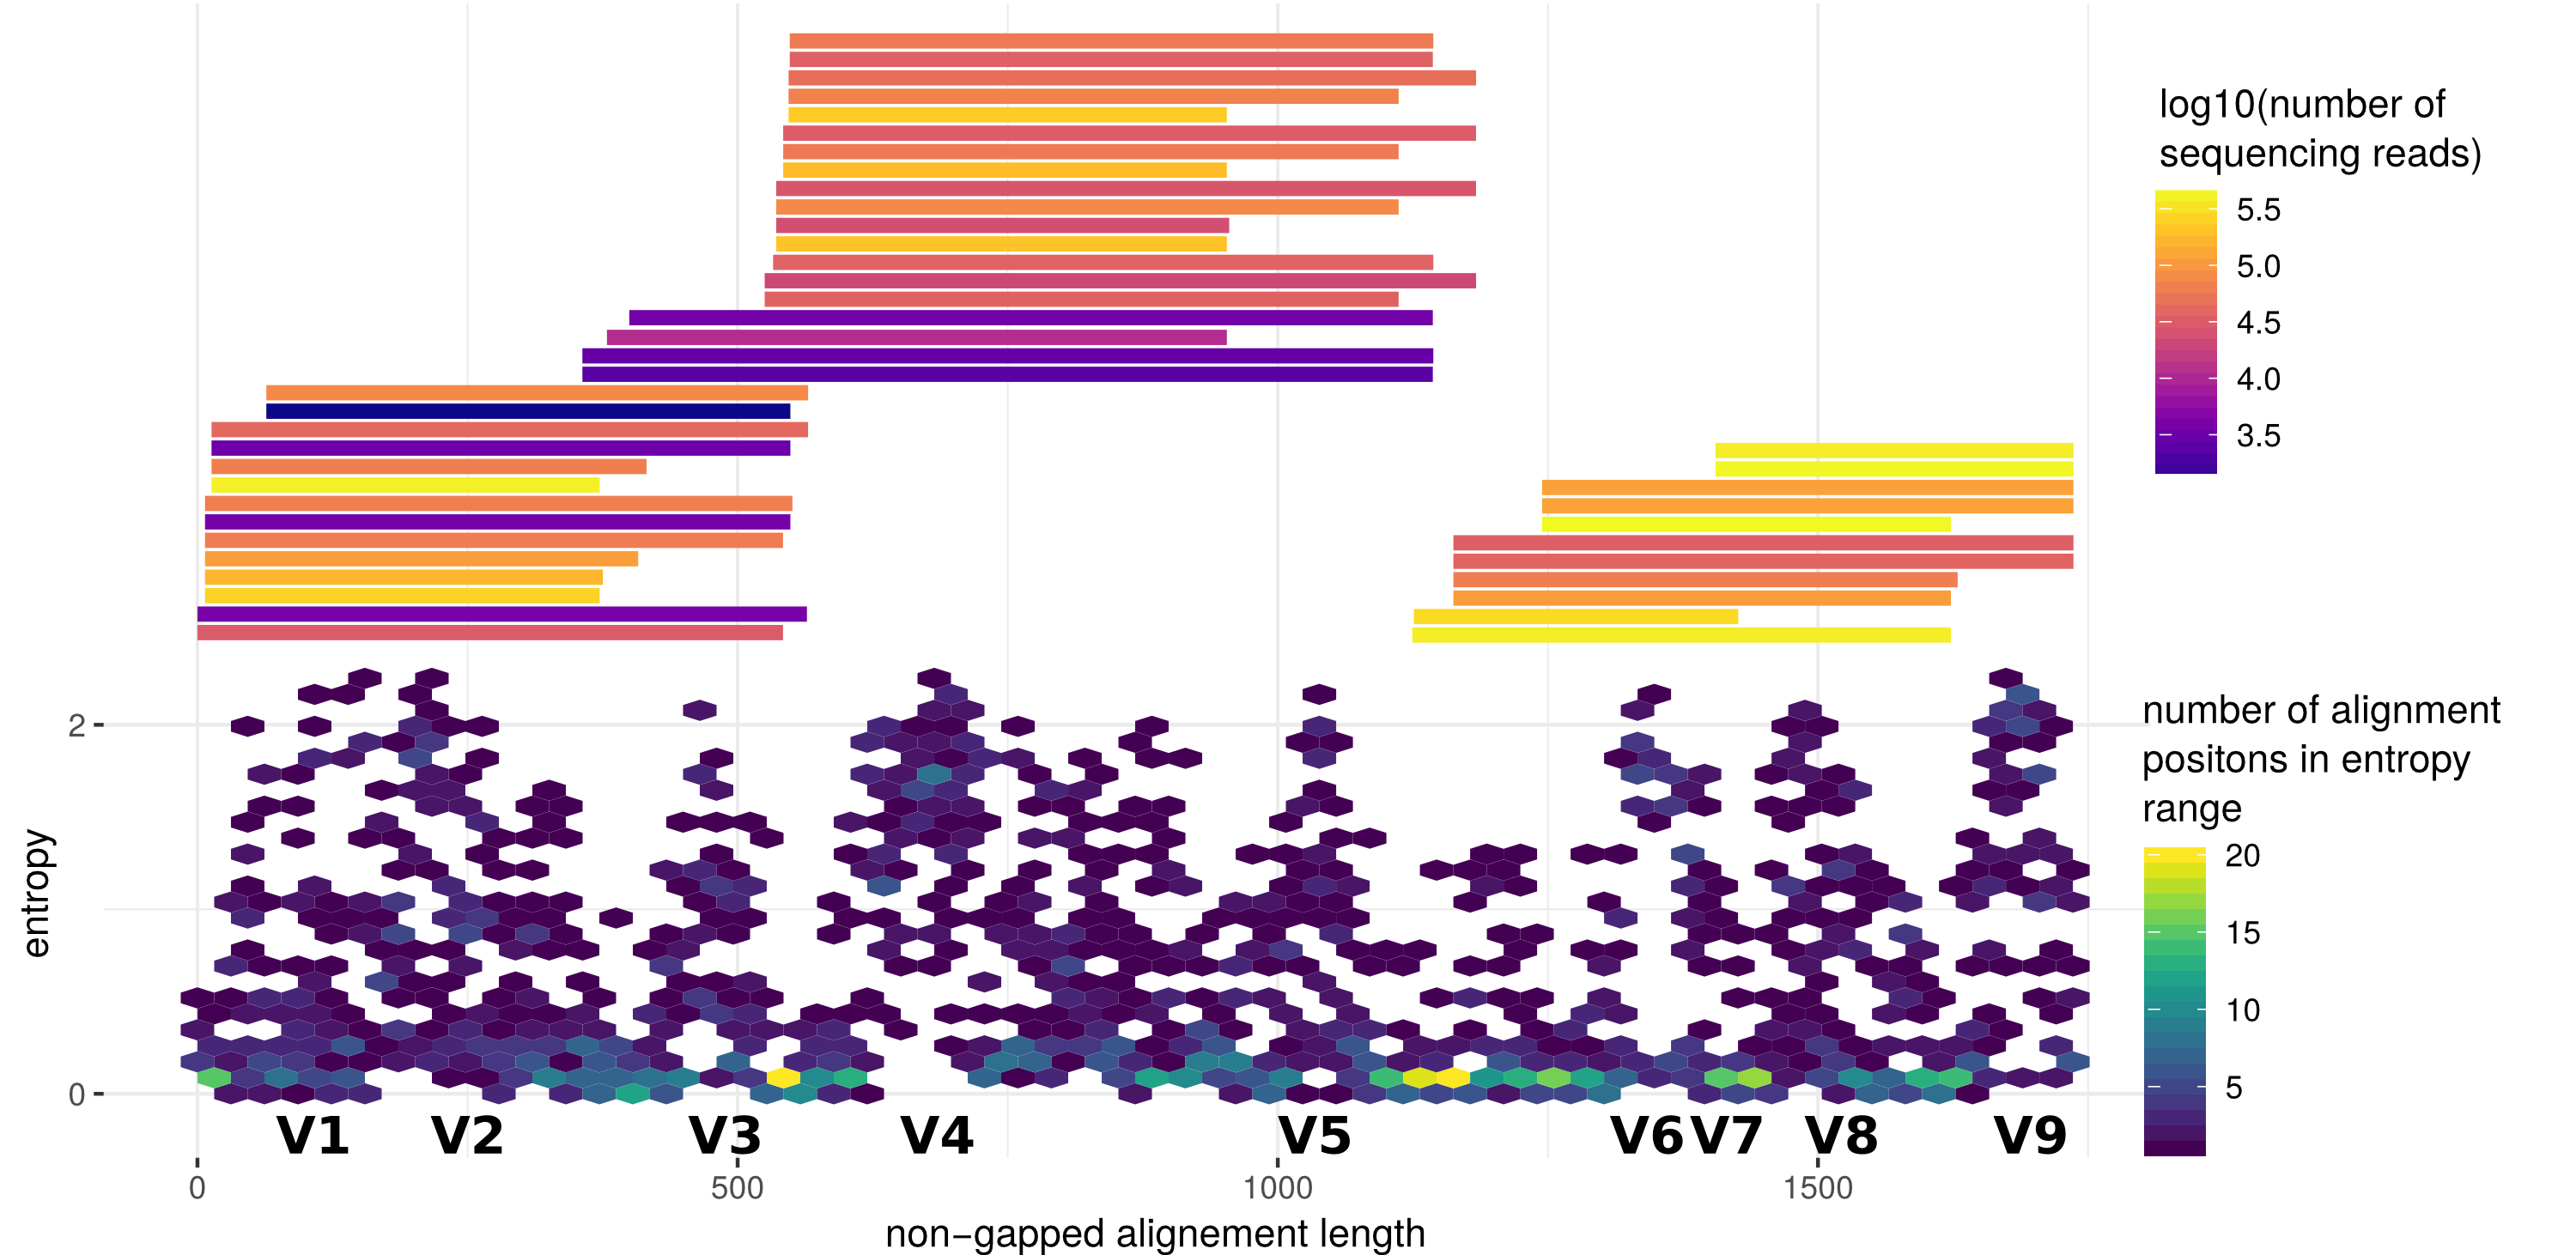
\includegraphics[width=1\linewidth]{entropy_primers_norm_woName.png}
        \textbf{Fig 2:} Amplicons used in this study in the context of
        entropy (evolutionary conservation and information content) of
        the eukaryotic 18S gene. Shannon entropy is displayed for the
        Silva reference alignment [3] of all eukaryotes. Primers were
        mapped against the same alignment. Positions along the gene
        are expressed as mean length of sequences (excluding gaps) for
        each column in the alignment.
      }

      
% ------------------------
% COLUMN 2 ---------------

\column{0.5}

\block{Summary}
{
    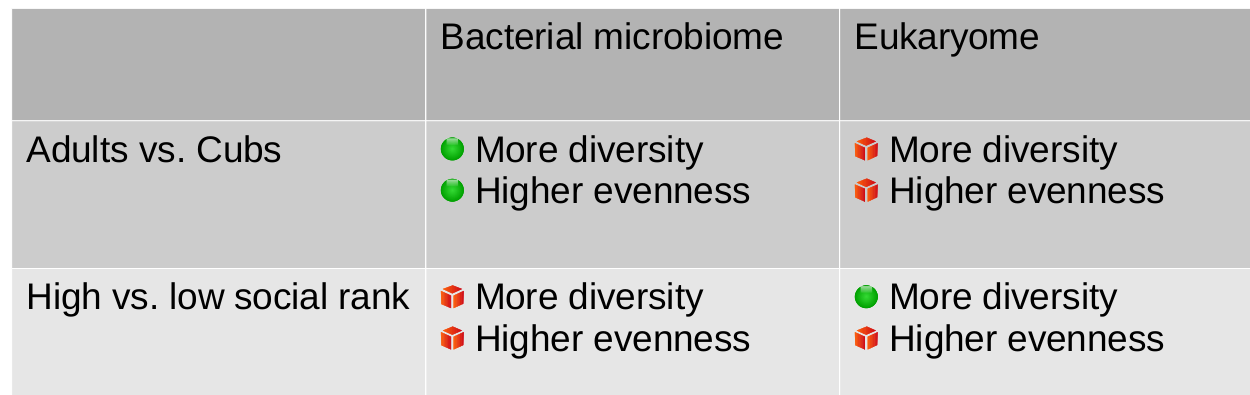
\includegraphics[scale=0.85]{summary.png}\\
    Green circles = Results matching predictions \hspace{1cm}
    Red squares = No confirmatory results
}

\block{Results: Bacterial microbiome} {

        \begin{minipage}{0.7\linewidth}                  
          \begin{left}
              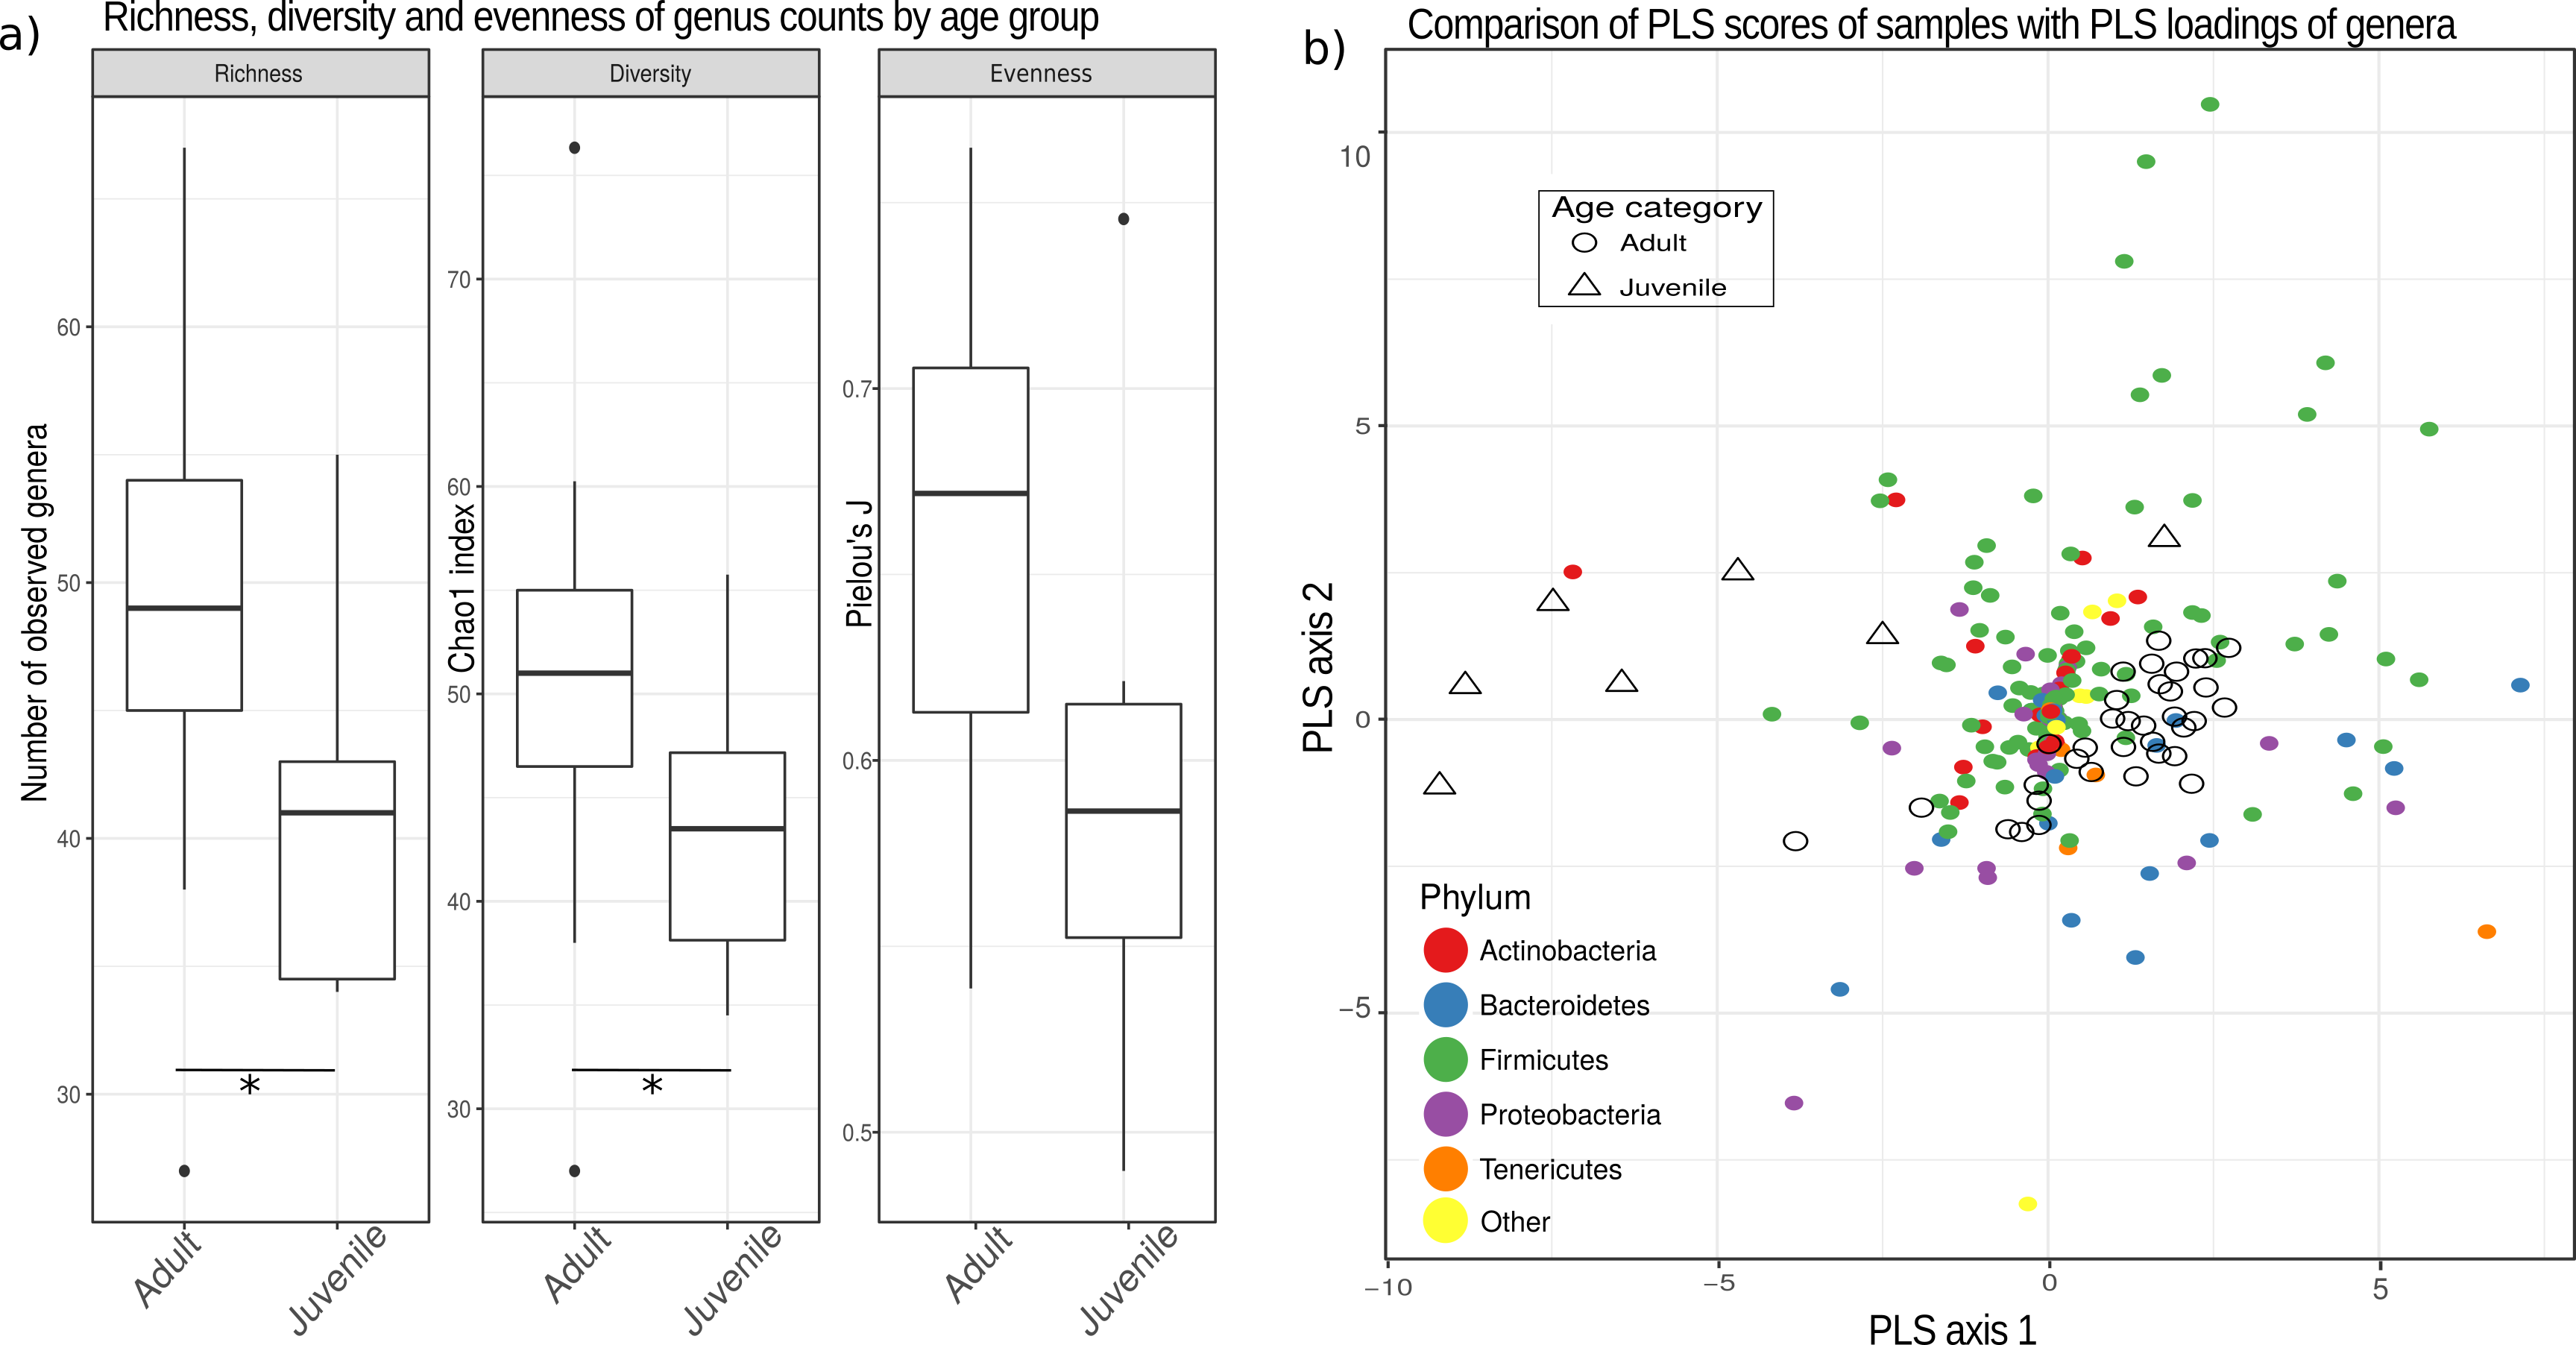
\includegraphics[scale=0.9]{Figure3_man.png} 
          \end{left}
        \end{minipage}
        \hfill
        \begin{minipage}{0.3\linewidth}
          \textbf{Fig 4:} a) Observed counts (richness) and diversity
          indices for genera are lower in juveniles compared to
          adults. b) Scores (for samples) and loadings (for genera) in
          a partial least squares model demonstrate differences in
          microbiome composition of adults and juveniles and highlight
          differently abundant taxa.\\
        \end{minipage}

        \\ $\Rightarrow$ \textbf{Adult female hyenas have a
          bacterial microbiome which is more diverse than and differs
          in composition from that of juveniles.}  }

\block{Results: Eukaryome} {
  \begin{minipage}{0.7\linewidth}                  
    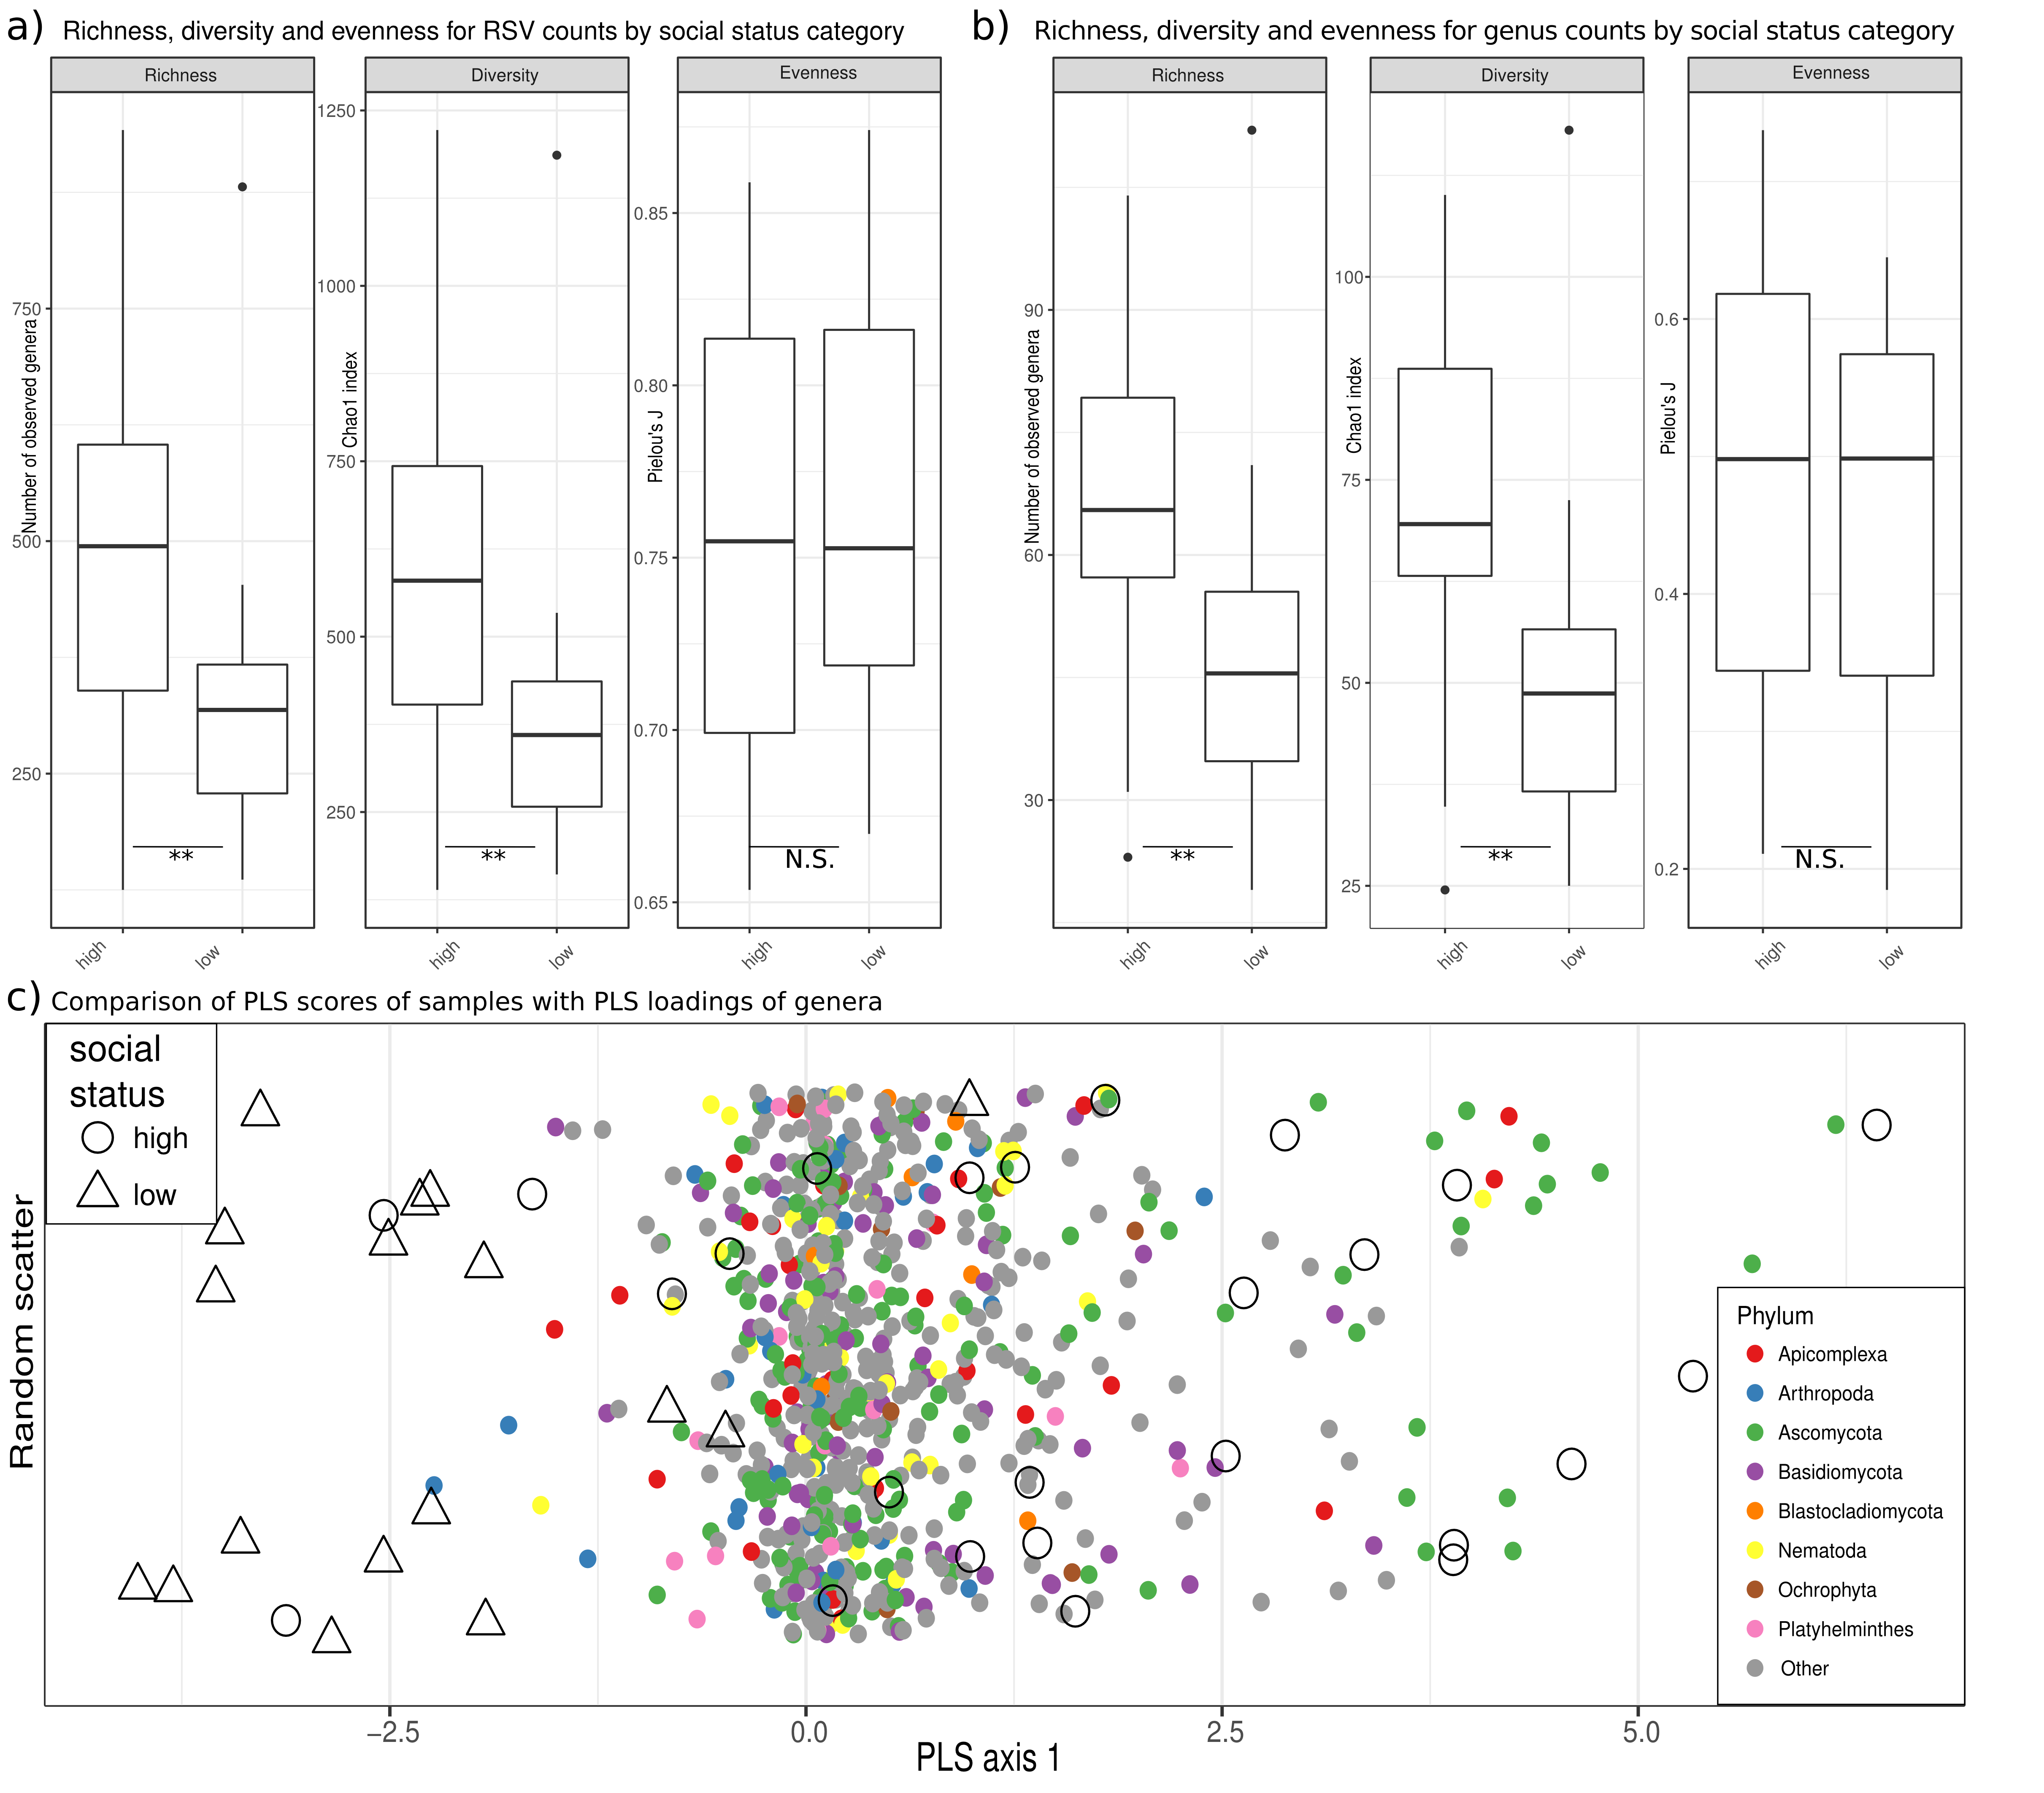
\includegraphics[scale=0.67]{Figure4_man.png}
  \end{minipage}
  \hfill
  \begin{minipage}{0.3\linewidth}
    \testbf{Fig 5:} Richness and diversity are higher for socially
    high compared to low ranking females, both at the level of a) RSVs
    b) genera.  c) PLS scores (for samples) and PLS loadings (for
    genera) on the single PLS axis of a model, separating the majority
    of samples from high-ranking individuals from samples from
    low-ranking animals.
  \end{minipage}
  $\Rightarrow$ \textbf{A more diverse eukaryome in high-ranking than
    low-ranking hyenas.} }


\block{Funding / Misc}
{

  The study was funded by the DFG Research Training Group 2046
  ``Parasite Infections: From Experimental Models to Natural Systems''
  (SCF) and Leibniz Institute for Zoo and Wildlife Research.

  \textbf{Published as:
  \hangindent=2cm  Heitlinger \textit{et al.} (2017) The
    Intestinal Eukaryotic and Bacterial Biome of Spotted Hyenas:
    The Impact of Social Status and Age on Diversity and
    Composition \textit{Front Cell Infect Microbiol. 7: 262.}}
}

\block{References}
      {
        \begin{small}

          \hangindent=2cm [1] Callahan \textit{et al.} (2016) DADA2:
          High-resolution sample inference from Illumina amplicon data
          \textit{Nature Methods} 13, 581--583

          \hangindent=2cm [2] Heitlinger (2017). MultiAmplicon version
          0.01 [R - package]. \textit{Zenodo}; Development version at
          https://github.com/derele/MultiAmplicon

          \hangindent=2cm [3] Pruesse \textit{et al.} (2007) SILVA: a
          comprehensive online resource for quality checked and
          aligned ribosomal RNA sequence data compatible with
          ARB. \textit{Nucleic Acids Research} 35:7188-7196

          
        \end{small}
      }

% ----------

\end{columns}

% ----------------
\end{document}
\endinput
%%
%% End of file 
